In der hochaufgelösten Resonanz-Ionisations-Spektroskopie ist es
sehr wichtig, über längere Messzeiten möglichst konstante Rahmenbedingungen für die Messung zu
schaffen. Auch die Reproduzierbarkeit von Messungen ist nur gewährleistet, wenn
die Experimentparameter konstant bleiben. Ein wesentlicher, wenn nicht der
wichtigste, Parametersatz des Experiments sind die Lasereigenschaften. Für
eine stabile Laserfrequenz ist die Stabilität des Resonators ausschlaggebend.
Vibrationen, Luftdichte- bzw. Verstärungsmediumsdichtefluktuationen und
Brechungsindexänderungen, hervorgerufen durch Temperaturschwankungen, sind für
Instabilitäten verantwortlich. Schon bei Schwankungen oder Drifts von wenigen
MHz kann es bei sehr schmalbandigen Atomaren Übergängen zu erheblichen
Fluktuationen in der Ionisatonsrate kommen. Daher ist eine aktive
Frequenzstabilisierung der Diodenlaser unerlässlich.\par
In diesem Kapitel sollen zunächst der Vollständigkeit halber bewährte
Frequenzstabilisierungstechniken wie
\textit{Hänsch-Couillaud} (Kap.
\ref{sec:haensch-couillaud}) und \textit{Pound-Drever-Hall} (Kap.
\ref{sec:pound-drever-hall}) kurz vorgestellt
(\cite{noertershaeuser:physik_des_lasers}) und anschließend auf das in diesem
Projekt verwendete \textit{Fringe-Offset-Locking} (Kap.
\ref{sec:fringe-offset-locking}) näher eingegangen werden. Darüber hinaus
besteht auch die Anforderung, zwischen den Anregungsfrequenzen verschiedener Isotope möglichst schnell wechseln zu können. Dies ist allein mit der Fringe-Offset-Locking nur bedingt gegeben. Deshalb wurde diese Technik mit einer kommerziellen Stabilisierunugstechnik kombiniert, auf die und deren Kombination mit der Fringe-Offset-Technik am Ende dieses Kapitals eingegangen wird.\par
Um einen Laser auf einer Frequenz festzuhalten, benötigt
man eine Referenz. Diese kann ein passiver, stabiler Resonator, ein atomarer
bzw. molekularer Übergang oder ein absolut stabiler Laser wie z.B. ein Helium-Neon-Laser sein.
Aus der Abweichung der Frequenz des zu stabilisierenden Lasers $\nu_{ist}$ zur
Sollfrequenz $\nu_{soll}$ muss ein Fehlersignal
\begin{equation}\label{eq:servoschleife_fehlersignal}
	S\approx C\cdot(\nu_{ist}-\nu_{soll})=C\cdot\delta\nu
\end{equation}
erzeugt werden, das hier exemplarisch linear zur Frequenzdifferenz $\delta\nu$
ist. Dieses Fehlersignal dient als Eingangssignal für eine Regelschleife, die
die Frequenz des Lasers auf die Sollfrequenz regelt. Auf Details dieser
Regelschleife soll später genauer eingegangen werden (siehe
\ref{sec:regeltechnik}). Die Generierung des Fehlersignals kann auf verschiedene Arten geschehen, wie im Folgenden zu sehen
ist.

\section{Hänsch-Couillaud}\label{sec:haensch-couillaud}
\begin{figure}[h]
 	\centering
 	\fbox{\parbox{\dimexpr \linewidth - 2\fboxrule - 2\fboxsep}{
 	\centering
	    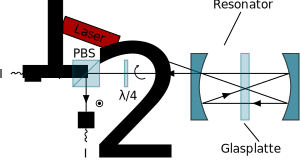
\includegraphics[width=\textwidth-4cm]{gfx/haensch-couillaud_aufbau}
	}}
	\caption[Hänsch-Couillaud - Aufbau]{Aufbau
	einer Frequenzstabilisierung nach Hänsch
	und Couillaud. Erkläung im Text.}\label{fig:haensch-couillaud_aufbau}
\end{figure}
Die Frequenzstabilisierung nach Hänsch und Couillaud (HC)
basiert auf der \textit{Polarisationsspektroskopie}. Mit Hilfe eines
optischen Elemtents in einem festen Resonators als Referenz können verschiedene
Polarisationen des Laserlichts verschiedene Verluste erfahren. Dies lässt sich
mit einem doppelbrechenden Kristall oder einer Glasscheibe im Brewsterwinkel
realisieren. Man kann das elektrische Feld des linear polarisierten einfallenden
Lichts $E_0$ in Komponenten senkrecht und parallel zur Polarisationsrichtung mit
minimalen Verlusten zerlegen:
\begin{equation}\label{eq:haensch-couillaud_01}
	\begin{split}
		E_{\perp}^{(0)} & = E_0\cdot\cos{(\Theta)}\\
		E_{\parallel}^{(0)} & = E_0\cdot\sin{(\Theta)}\,.
	\end{split}
\end{equation}
Dabei ist $\Theta$ der Winkel zwischen einfallender Polarisation und
Polarisation mit maximalen bzw. minimalen Verlusten. $E_{\perp}^{(0)}$ wird also
im Wesentlichen vom Einkoppelspiegel reflektiert. $E_{\parallel}^{(0)}$
wird hingegen in den Resonator eingekoppelt und erfärt bei Nicht-Resonanz im
Resonator eine Phasenverschiebung $\delta$ zu $E_{\perp}^{(0)}$. Im Resonanzfall
ist diese Phasenverschiebung null. Durch Kenntnis der Phasenverschiebung kann
also eine Aussage über die Verstimmung zur Resonanz getroffen werden. Die
Komponenten des refelktierten Lichts
\begin{equation}\label{eq:haensch-couillaud_02}
	\begin{split}
		E_{\perp}^{(r)} & = E_{\perp}^{(0)}\cdot r_1\\
		E_{\parallel}^{(r)} & = E_{\parallel}^{(0)}\cdot\left(r_1-\frac{t_1^2r\mathrm{e}^{-\mathrm{i}\delta}}{r_1\left(1-r\mathrm{e}^{-\mathrm{i}\delta}\right)}\right)
	\end{split}
\end{equation}
ergeben zusammen elliptisch polarisiertes Licht und somit eine Überlagerung von
$\sigma^+$- und $\sigma^-$-Licht mit unterschiedlichen Amplituden. Dabei sind
$r_1$ und $t_1$ Reflexions- und Transmissionskoeffizienten des
Einkoppelspiegels. $r$ beschreibt die Verluste durch die Umläufe im Resonator.
Bei Phasenverschiebung überwiegt einmal der $\sigma^+$-Anteil und einmal der $\sigma^-$-Anteil. Bei Resonanz sind beide Anteile gleich und es entsteht wieder linear polarisiertes Licht. Eine $\nicefrac{\lambda}{4}$-Platte erzeugt aus
beiden zirkularen Anteilen ($\sigma^+$ und $\sigma^-$) lineare Anteile, welche
durch einen Polarisationsstrahlteiler getrennt und letzendlich durch Photodioden
detektiert werden können. Abbildung \ref{fig:haensch-couillaud_aufbau} zeigt den
optischen Aufbau. Die Differenz der zu den Feldstärken der elektrischen Komponente
des Lichts proportionalen Ströme der Photodioden
\begin{equation}\label{eq:haensch-couillaud_fehlersignal}
	(I_1-I_2)\propto\abs{E^{(0)}}^2\cos{(\Theta)}\sin{(\Theta)}\frac{t_1^2r^2\sin{(\delta)}}{(1-r^2)+4r^2\sin^2{\left(\frac{\delta}{2}\right)}}
\end{equation}
lieftert das in Abb. \ref{fig:haensch-couillaud_fehlersignal} gezeichnete
Fehlersignal mit Nulldurchgang bei den Resonanzen $\delta=2\pi n$. Die
Regelschleife muss also auf diesen Nulldurchgang regeln.
\begin{figure}[h]
	\centering
	\footnotesize
	\input{plt/haensch-couillaud_fehlersignal}
	\caption[Hänsch-Couillaud
	Fehlersignal]{Fehlersignal der
	Hänsch-Couillaud-Stabilisierung
	gemäß Gl.
	\eqref{eq:haensch-couillaud_fehlersignal}.
	Der markierte Bereich ist der
	Fangbereich der Regelung.}\label{fig:haensch-couillaud_fehlersignal}
\end{figure}

\section{Pound-Drever-Hall}\label{sec:pound-drever-hall}
\begin{figure}[h]
 	\centering
 	\fbox{\parbox{\dimexpr \linewidth - 2\fboxrule - 2\fboxsep}{
 	\centering
	    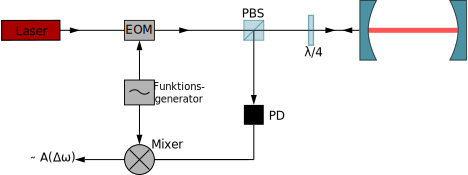
\includegraphics[width=\textwidth-0.5cm]{gfx/pound-drever-hall_aufbau}
	}}
	\caption[Pound Drever Hall - Aufbau]{Aufbau
	einer Frequenzstabilisierung nach Pound, Drever und Hall. Erkläung im
	Text.}\label{fig:pound-drever-hall_aufbau}
\end{figure}
Ein Aufbau des Verfahrens nach Pound, Drever und Hall (PDH) ist in Abb.
\ref{fig:pound-drever-hall_aufbau} dargestellt.
Das Laserlicht mit der Frequenz $\omega_L$ wird mittels eines \textit{elektrooptischen Modulators}, kurz EOM, in der Phase gemäß
\begin{equation}\label{eq:pound-drever-hall_01}
	E=\E_0\cos{\left(\omega_Lt+\delta\cos{(\omega_mt)}\right)}
\end{equation}
mit einem kleinen Modulationsindex $\delta\ll1$ moduliert. Dabei treten in
erster Ordnung gegenphasige Seitenbänder mit der Frequenz $\omega_L\pm\omega_m$
auf. Als Referenz dient wieder wie oben ein Resonator, in den bei Resonanz ein
Teil des Trägerlichts eingekoppelt wird. Die Seitenbänder und der restliche Teil
des Trägers werden refelektiert. Da bei Resonanz das Licht im Resonator einen
Phasensprung von $\pi$ erfährt, ergibt sich für die Nettoleistung des
refelktierten Trägerlichts eine Abschwächung durch destruktive Interferenz.
Da die beiden Seitenbänder gegenphasig schwingen, haben die Schwebungen dieser
Seitenbänder mit dem Träger unterschiedliche Vorzeichen. Im Resonanzfall heben
sich also die Schwebungssignale aufgrund gleicher Amplitude gegenseitig auf, was
zu vollständiger destruktiver Interferenz führt. Bei geringer Verstimmung des
Lasersfrequenz zur Resonanzfrequenz des Resonators, ist die Phasenverschiebung
im Resonator nicht mehr $\pi$, was zu unterschiedlichen Amplituden der
Schwebungssignale führt. Das resultierende Signal ist also von null
verschieden.\par
Die Trennung des einfallenden Lichts vom zu analysierenden Licht kann mit einer
$\nicefrac{\lambda}{4}$-Platte und einem Polarisationsstrahlteiler realisiert
werden. Für den Photodiodenstrom erhält man in Abhängigkeit von der Verstimmtung
des Trägerlichts zur Resonanz
\begin{equation}\label{eq:pound-drever-hall_fehlersignal}
	I(\Delta\omega,\omega_m)\propto
	J_0(\delta)J_1(\delta)\left[A(\Delta\omega)\cos{(\omega_mt)}+D(\Delta\omega)\sin{(\omega_mt)}\right]\,,
\end{equation}
wobei $J_{0,1}$ nullte und erste Ordnung von Besselfunktionen sind. Mischt man
das Signal mit dem der Modulation, erhält man als Ausgangssignal den zur
Modulation gleichphasigen Anteil von
Gl. \eqref{eq:pound-drever-hall_fehlersignal}, der proportional zu
$A(\Delta\omega)$ ist.
Abbildung \ref{fig:pound-drever-hall_fehlersignal} zeigt die Abhängigkeit dieses
Fehlsignals zur Verstimmung $\Delta\omega$. Um den Laser auf Resonanz zu halten,
muss auf den Nulldurchgang geregelt werden.
\begin{figure}[h]
	\centering
	\footnotesize
	\input{plt/pound-drever-hall_fehlersignal}
	\caption[Hänsch-Couillaud
	Fehlersignal]{Fehlersignal der
	Pound-Drever-Hall-Stabilisierung
	gemäß Gl.
	\eqref{eq:pound-drever-hall_fehlersignal}. Die Modulation 
	$\pm\omega_m$ liegt bei $\pm5$.}\label{fig:pound-drever-hall_fehlersignal}
\end{figure}

\section{Fringe-Offset-Locking}\label{sec:fringe-offset-locking}
Die oben erklärten Techniken sind darauf ausgelegt einen einzigen Laser zu
stabilisieren. Ein Frequenzscan ist bei der PDH-Methode nur sehr eingeschränkt
möglich. Der Referenz-Resonator müsste sehr langsam verstimmt werden, damit die
Regelung nach kommt. Größere Frequenzsprünge sind auch bei der HC-Methode auch
nur bedingt möglich. Hier wird allerdings eine Stabilisierung benötigt, die drei
Laser unabhängig voneinander kontrollieren kann. Schnelles Verfahren auf
gewünschte Relativfrequenzen sind auch gefordert. Aus Kosten- und
Aufwandsgründen ist es auch von Vorteil, wenn für alle drei Laser dieselbe
Referenz verwendet werden können, ohne, dass sie voneinander abhängig sind. Eine
hervorragende Methode dafür ist das Fringe-Offset-Locking. Diese Methode soll im
Folgenden genauer betrachtet werden.

\subsection{Fabry-Perot-Interferometer}
Eine entscheidende Rolle spielt hier ein sog.
\textit{Fabry-Perot-Interferometer}, kurz FPI, das sowohl
als feste Referenenz als auch als Frequenzspektrum-Analysator dienen kann.
Beide Varianten sollen in diesem Kapitel vorgestellt werden.

\subsubsection{Festes FPI}

